\documentclass[]{scrartcl}
\usepackage{graphicx}
\graphicspath{{../CMS_Plots/}, {../CMS_Events/}, {../CMS_Scatter/}}
%opening
\title{Thesis Draft}
\author{Jerrod Dixon}

\begin{document}

\maketitle

\section{Introduction}
Implemented internationally, the Worldwide LHC Computing Grid (WLCG) operates as a conglomeration of computing centers managed by universities. The goal is to cooperate in processing the large amounts of data (~50 Petabytes in 2016 alone) produced by the Large Hadron Collider (LHC) at CERN.

Over the years, the processing methods have improved, and the implementation of the WLCG itself has grown in such a way that more data is produced than can be processed in a reasonable amount of time. This has resulted in backlogs of data requiring processing. Coordination of work is at issue as well, deciding when and where the transfer of the data to offsite locations should occur and where it is to go. 

Depending on which labs require the dataset, the data can be replicated in multiple geographically distant locations in such a way to allow easier access. Also, load balancing of work causes issues with users submitting work to be done to the same processing center. This can cause certain locations to become overloaded with requests for processing while others go almost unused. By extension the data also runs into the issue of being requested to do the calculations against getting called to a processing center that is not geographically close, for example the job is processed in Italy but the data exists in Spain, slowing the acquisition time. 

\section{Background}
A grid network is classically defined as a software solution, implementing general commodity hardware, to enable the creation of a series of machines to achieve High Performance Computing (HTC). The benefit here, is that by implementing such a solution, allows for cheaper access to HTC style computing without requiring investment into designing and implementing specialized hardware to improve scientific computations.

In HTC solutions, following the previous definition, there are times when the cluster is not fully in use by the institution that developed it. Because of this, institutions across the globe have come up with methods to connect their personal clusters to a international grid. In this way, these HTC solutions are better utilized to achieve a higher usage saturation point, taking work from excessively busy systems and giving work to idle ones.

\subsection{WLCG Network Grid}
CERN laboratories have used this model of computation to implement their own international grid network, the WLCG. Via this grid, data produced by experiments performed at CERN with the Large Hadron Collider (LHC) can be sent offsite not only for storage of the data but for processing as well. The type of data produced in these experiments are of such an architecture, that standard processing methods such as utilizing a single machine are not sufficient to process the data in a reasonable amount of time. By using this HTC style of computing the data can be processed in a significantly shorter duration.
\subsubsection{Involved Facilities}
\subsubsection{CMS Experiment}
\subsection{Nature of WLCG jobs}
\subsubsection{Condor}
\subsubsection{Important Properties}
\subsection{Importance of reported values}
\subsection{Motivation}

\section{Related Work}
\subsection{Atlas MWT2}
\subsubsection{Elasticsearch}
\subsubsection{PerfSONAR}
\subsection{Cern CMS experiment}

\section{Experiment on CMS performance}
\subsection{Setup}
The raw data exists in two locations. The data containing job performance values(?need a better word?) is located and stored at hcc-metrics.unl.edu in an Elasticsearch database. The data stored there is obtained via python script, querying the Condor adclass databases of every cluster that runs in the WLCG network. Most values obtained are raw and straight from the databases while others, such as the frequently used CpuEff statistic, are calculated from the raw values. Elasticsearch is used as it provides a light and fast method of storing and querying the data in a non-relational method.

The data related to network performance across data links is also stored in an Elasticsearch server, but as part of an Atlas MWT2 installation. The data is collected individually, using perfSONAR systems setup at specified locations to gather data about packet loss, latency, and throughput across certain links. The word 'certain' used here as perfSONAR systems are not widely implemented so there are limited sites where meaningful values can be obtained from.
\subsubsection{Aggregation of Condor databases}
\subsubsection{Elasticsearch Servers}
These two datasets are the ones we are interested in looking at, but first the values need to be joined together to make relational arguments. This is made difficult for multiple reasons. The first being that the network data from MWT2 is not specified on a per job basis, only an aggregation of all work over a period of time. Secondly, names of locations are not similar between databases. As a result a local json 'stitching' file is used to equate name values from one dataset with the other. 

To cover the difficulty of the first issue, that being the data is an aggregation, the data is taken from both sets paying attention to the JobStart and JobComplete date values of the hcc-metrics dataset. If the date of collection in the MWT2 database (networking information) overlaps with the period of running for the job, then the two datasets are considered to be 'matched' in that moment. An aggregation of that date period is done with all jobs that are satisfied by the 'valid' date of the network information, then averaged and split into ten minute chunks. This data is then stored on a third privately controlled Elasticsearch server.
\subsubsection{Processing method of data}
\section{Results}
\subsection{Effects on job performance}
\subsection{Packet Loss}
\begin{figure}
	\caption{Changes in CpuEff and EventRate over time pre-processing}
	\centering
	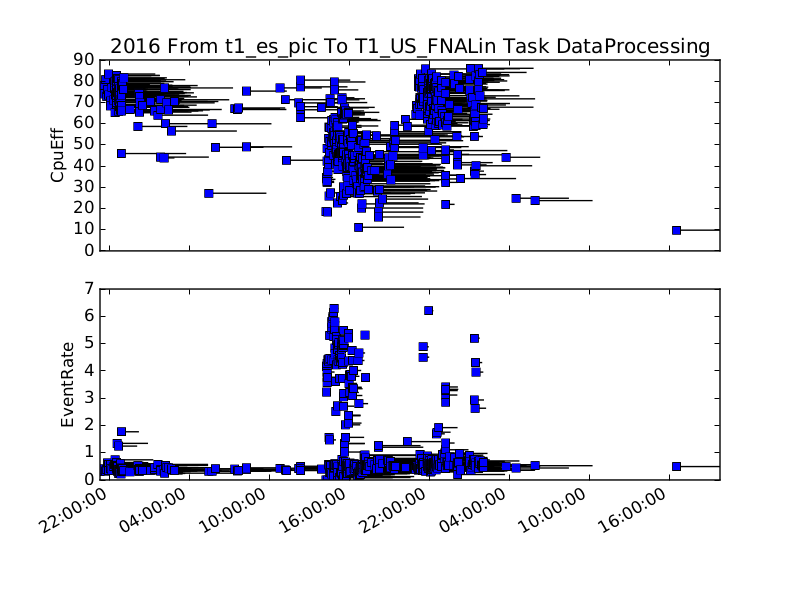
\includegraphics[scale=0.5]{CpuEff_EventRate_pic_FNAL}
\end{figure}
\begin{figure}
	\caption{Changes in CpuEff and EventRate over packet loss post-processing}
	\centering
	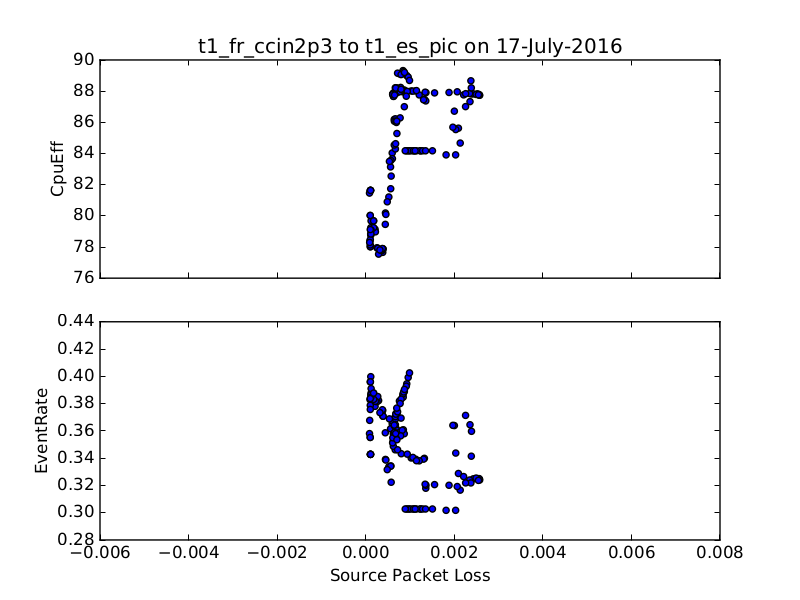
\includegraphics[scale=0.5]{EventRate_CpuEff_ccin2p3_pic_packet}
\end{figure}
\subsection{Latency}
\begin{figure}
	\caption{Changes in CpuEff and EventRate over latency registered from source site}
	\centering
	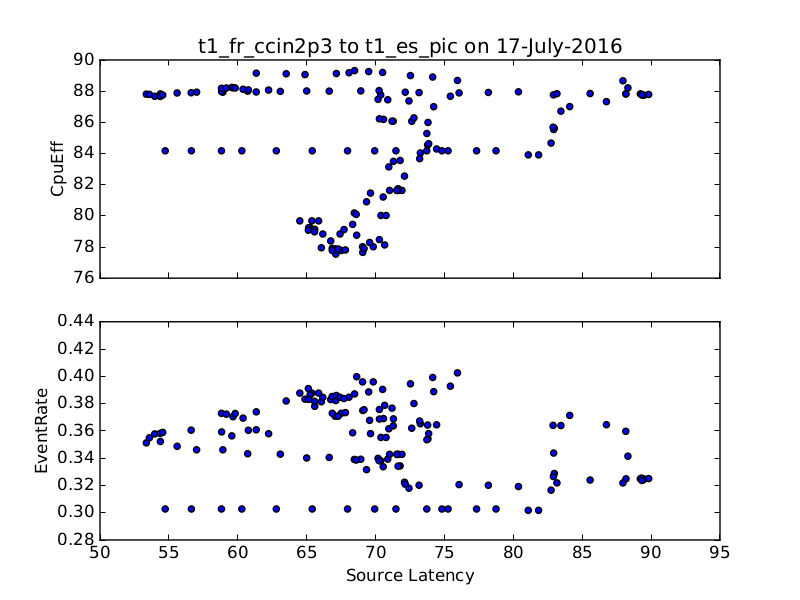
\includegraphics[scale=0.35]{EventRate_CpuEff_ccin2p3_pic}
	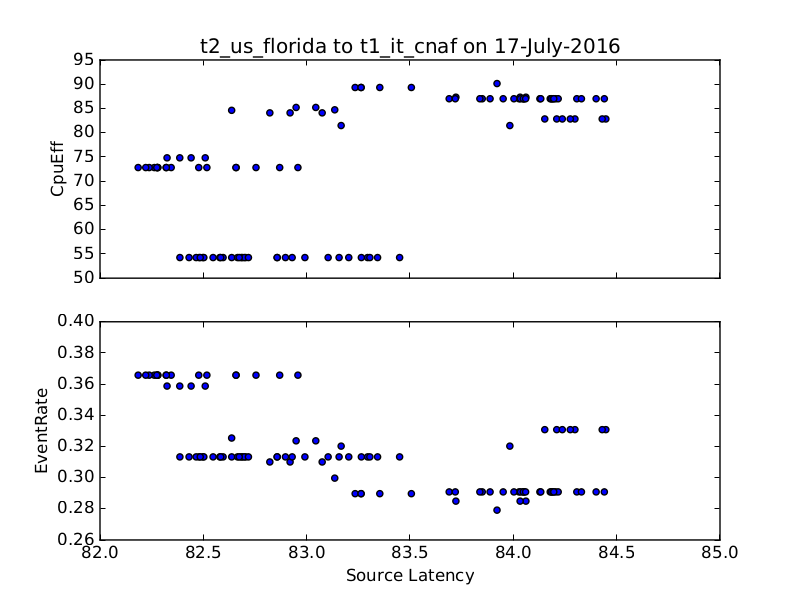
\includegraphics[scale=0.35]{EventRate_CpuEff_florida_cnaf}
	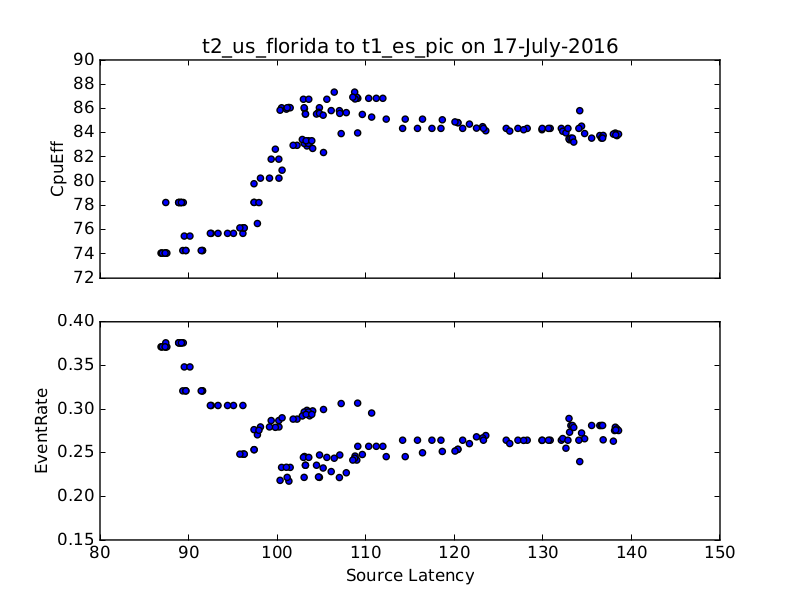
\includegraphics[scale=0.35]{EventRate_CpuEff_florida_pic}
\end{figure}
\subsection{Throughput}
\subsection{Issues with data}
\begin{figure}
	\caption{Some data 'stalagmites' and am unsure of its meaning}
    \centering
	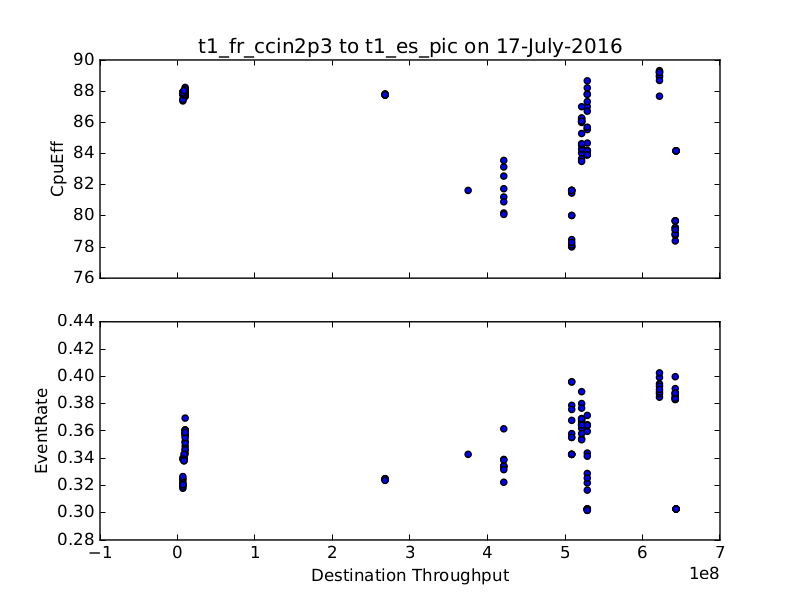
\includegraphics[scale=0.3]{EventRate_CpuEff_ccin2p3_pic_dest_through}
	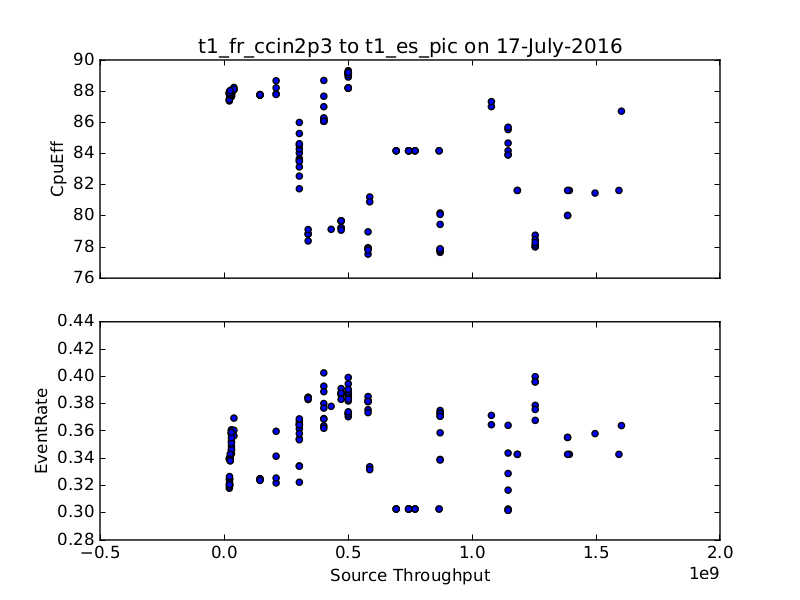
\includegraphics[scale=0.3]{EventRate_CpuEff_ccin2p3_pic_through}
\end{figure}

\section{Conclusions and Future Work}
\subsection{Side discoveries}
\subsubsection{Drop in EventRate against CpuEff}
\end{document}
